\section{Processo implementativo}
\label{sec:chapter_3_section_5}

Con processo di implementazione dei \emph{Plugin} si intende la formalizzazione in modo dettagliato le fasi seguite.
Il processo è scindibile principalmente nelle seguenti fasi:
\begin{itemize}
  \item ricerca delle specifiche del plugin
  \item definizione funzione 2D
  \item definizione funzione 3D
  \item instanziamento nel catalogo del nuovo plugin
  \item test del plugin con inserimento nella scena
\end{itemize}

\subsection*{Plugin Catalog}
\label{sec:chapter_3_section_5_sub_1}

\noindent
 Il plugin catalog \`e l'elemento centrale che fornisce allo users un sistema con un ricco catalogo di plugins,
 in cui, ogni elemento presente al suo interno \`e descritto da un nome, una descrizione ed una
 immagine di anteprima del modello 3D (come si vede in Figura~\ref{fig:figura1} (a)). Quando l'utente \`e al suo interno
 sceglie il plugin da inserire con un click, dopo il quale, si passa nella modalit\`a 2D-view, dove verr\'a posizionato
 all'interno della scena (come si vede in Figura~\ref{fig:figura1} (b)).


\begin{figure}[htbp]
\begin{center}
\begin{tabular}{c @{\hspace{1em}} c}
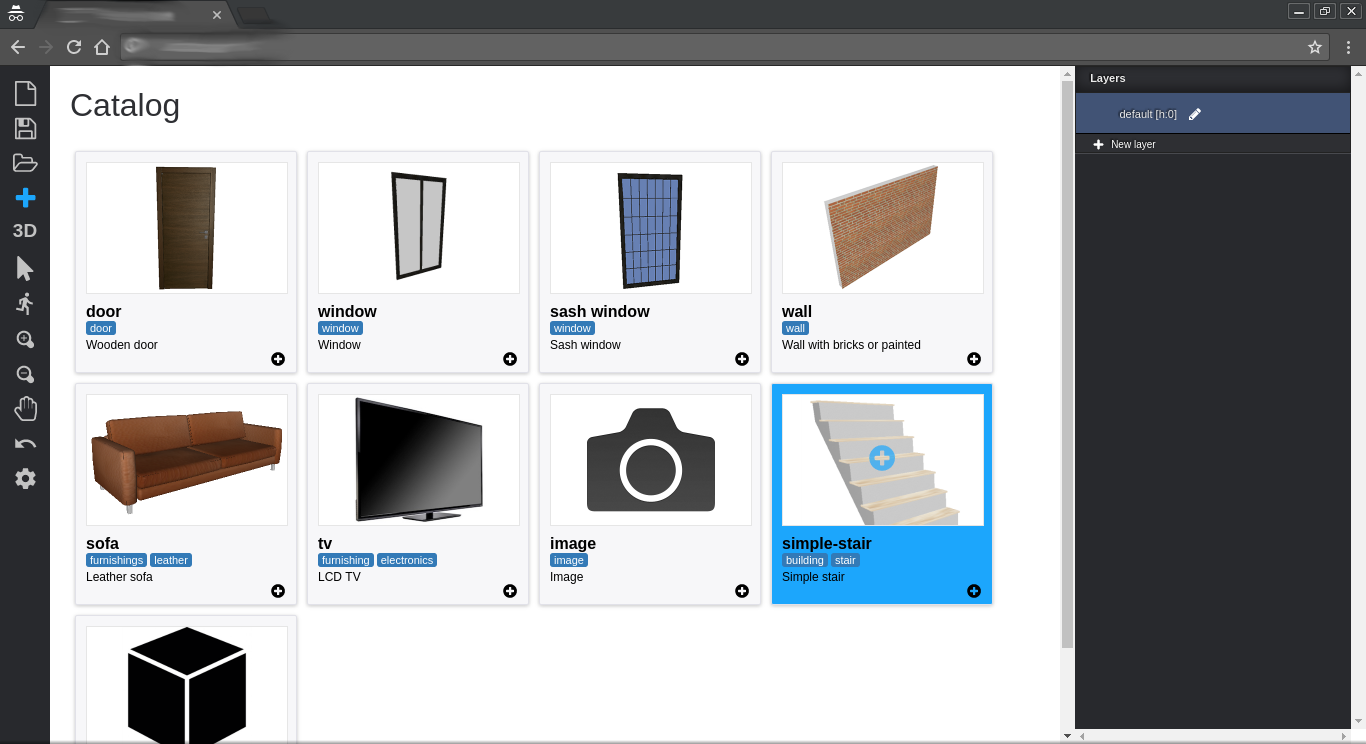
\includegraphics[width=9cm]{images/figcatalog} \\
  (a)  \\
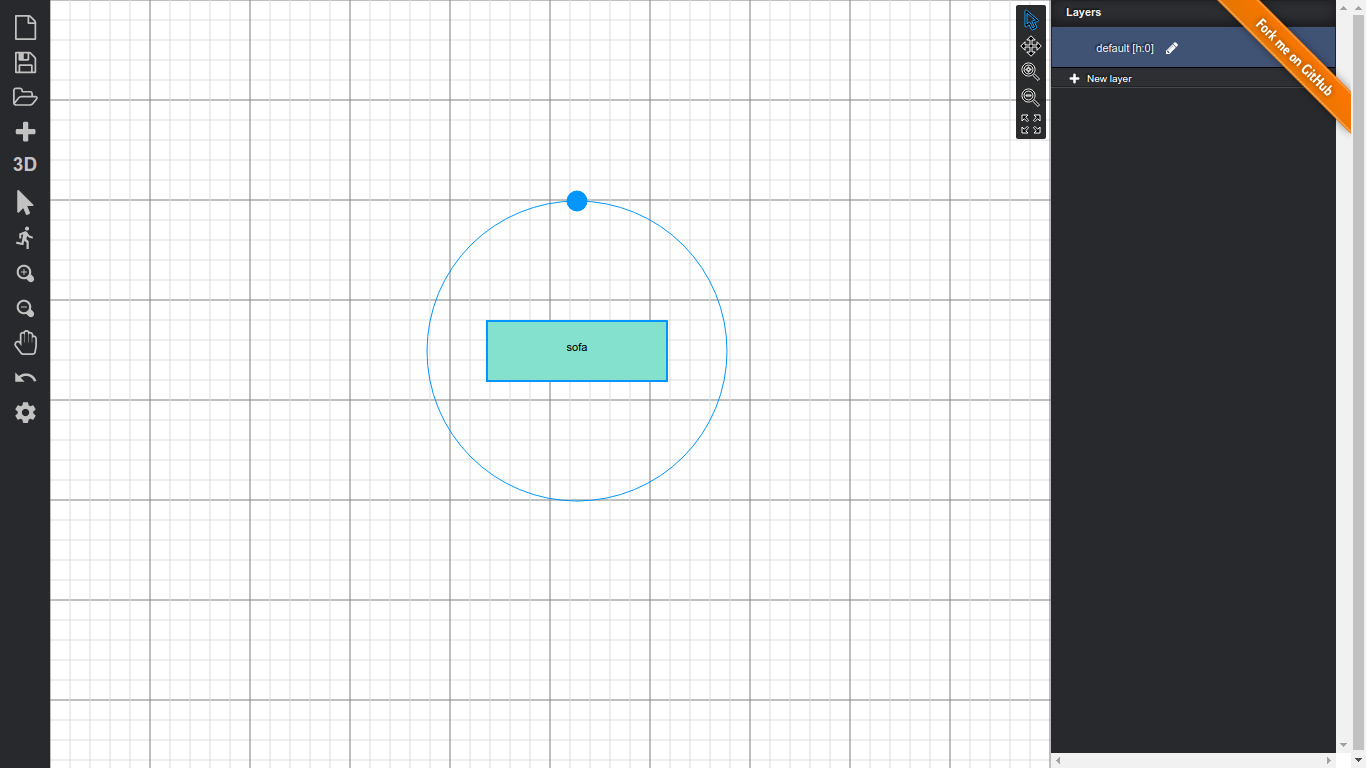
\includegraphics[width=9cm]{images/positioning} \\
  (b) \\
\end{tabular}
\end{center}
\caption{Dettaglio Plugins: (a) Vista dei plugins nel catalogo, (b) inserimento oggetto dopo la selezione nel catalogo}\label{fig:figura1}
\end{figure}
\newpage
